\chapter*{Introducción}\label{chapter\:introduction}


\textit{Gaussian Splatting} [\cite{kerbl20233d}] es una técnica innovadora que ha revolucionado recientemente el campo del renderizado y la reconstrucción tridimensional, 
ofreciendo una forma eficiente y precisa de visualizar escenas complejas con gran realismo. 
Este método se basa en representar los objetos y entornos mediante la superposición de pequeñas distribuciones gaussianas tridimensionales que, 
al combinarse, logran capturar detalles visuales sutiles y texturas realistas con una alta fidelidad. 
Gracias a su capacidad de generar representaciones visualmente convincentes con tiempos de ejecución considerablemente inferiores a 
otras técnicas previas, el \textit{Gaussian Splatting} se ha convertido rápidamente en uno de los métodos más adoptados en aplicaciones 
que requieren la visualización dinámica y precisa de entornos reales o virtuales.

Sin embargo, aunque sus aportes son indiscutibles, aún existen ciertos desafíos que limitan su plena eficacia, especialmente en situaciones que 
demandan altos niveles de precisión geométrica y fidelidad visual extrema. Estos retos motivan la búsqueda de soluciones innovadoras que permitan 
superar las limitaciones actuales, ampliando así el potencial del \textit{Gaussian Splatting} y consolidando su posición como herramienta clave en 
un espectro aún más amplio de aplicaciones tecnológicas y científicas. Esta tesis aborda precisamente estos desafíos, proponiendo mejoras que 
incrementen la calidad y precisión del método sin comprometer su eficiencia computacional ni la adaptabilidad a investigaciones existentes.

\section{Motivación}
\textit{Gaussian Splatting (GS)} [\cite{kerbl20233d}] se ha consolidado recientemente como uno de los métodos más efectivos para la representación y 
visualización eficiente de escenas tridimensionales. La relevancia del GS se evidencia en la adopción generalizada 
de este framework en trabajos recientes [\cite{ chen2024survey}] que abordan desde reconstrucciones dinámicas en cuatro dimensiones hasta representaciones volumétricas complejas. 
Sin embargo, a pesar de sus ventajas, GS presenta limitaciones importantes relacionadas con la forma subóptima adoptada por las gaussianas durante el 
entrenamiento. Diversos estudios han demostrado que estas gaussianas tienden a degenerar en formas anisotrópicas dominadas por una sola varianza, 
lo que genera artefactos en forma de aguja, geometrías subóptimas y normales inexactas [\cite{hyung2024effectiverankanalysisregularization, huang2024spectralgstaming3dgaussian,yu2023mipsplattingaliasfree3dgaussian}]. 
Esto surge de la incapacidad inherente del GS para modelar adecuadamente discontinuidades y límites definidos 
debido a la naturaleza continua de las distribuciones gaussianas [\cite{qu2024discgsdiscontinuityawaregaussiansplatting}]. Por tanto, surge 
la necesidad de investigar nuevas alternativas para mejorar estas limitaciones sin afectar significativamente la estructura general del método
para que pueda ser adaptado a otras investigaciones ya existentes.

\section{Problemática}
La técnica de \textit{Gaussian Splatting} ha demostrado ser una herramienta poderosa para la representación de escenas tridimensionales complejas,
sin embargo, a pesar de su eficacia general, se han identificado una serie de limitaciones fundamentales que comprometen su rendimiento 
en escenarios reales, especialmente en aquellos donde se requiere una alta fidelidad en los detalles geométricos y visuales.

\begin{figure}[htbp]
    \centering
    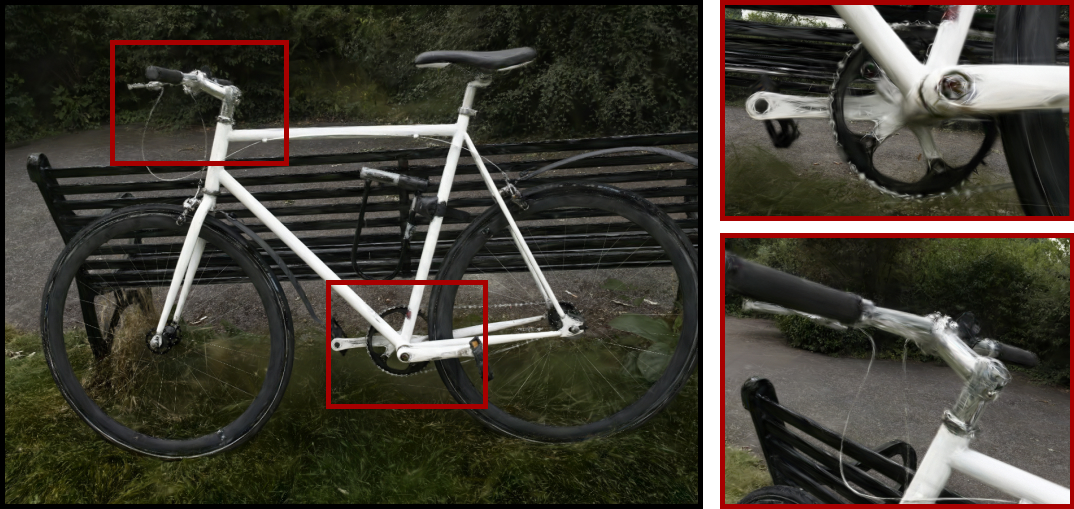
\includegraphics[width=0.9\textwidth]{Graphics/bici.jpg}
    \caption{Ejemplo visual de artefactos tipo ''aguja'' generados por la degeneración anisotrópica de gaussianas en \textit{Gaussian Splatting}. 
    En ambas ampliaciones se evidencia cómo ciertas 
    gaussianas adquieren formas extremadamente alargadas en direcciones específicas, generando artefactos visuales notorios que degradan 
    significativamente la calidad visual y comprometen la precisión geométrica de la reconstrucción.}
    \label{fig:bici}
\end{figure}

Una de las principales problemáticas asociadas al \textit{Gaussian Splatting} es la tendencia de las gaussianas a adquirir formas altamente anisotrópicas 
durante el proceso de optimización. Esto significa que, en lugar de mantener una forma más esférica o moderadamente elipsoidal, las gaussianas 
tienden a elongarse excesivamente en una dirección específica debido a una varianza dominante, generando artefactos visuales conocidos como agujas. 
Este comportamiento, reportado en estudios recientes  [\cite{hyung2024effectiverankanalysisregularization, huang2024spectralgstaming3dgaussian, yu2023mipsplattingaliasfree3dgaussian}],
no solo degrada la calidad visual de la reconstrucción, sino que también compromete la precisión de las normales estimadas, lo cual es crítico 
en tareas de iluminación realista y renderizado de alta calidad.
Además de esta degeneración geométrica, existe otra limitación importante: la incapacidad inherente del modelo para representar adecuadamente 
bordes abruptos, discontinuidades o superficies con cambios de curvatura pronunciados. Esta deficiencia proviene del hecho de que las gaussianas 
son distribuciones continuas por naturaleza, lo que las hace poco adecuadas para capturar transiciones bruscas en los datos visuales. Este fenómeno 
ha sido discutido en trabajos como \cite{qu2024discgsdiscontinuityawaregaussiansplatting}, donde se señala explícitamente que el 
uso exclusivo de gaussianas limita la capacidad del modelo para representar bordes definidos, afectando negativamente la reconstrucción 
de objetos con geometría compleja o detalles finos.

Cabe señalar que estas limitaciones no solo afectan la calidad visual, sino que también restringen la aplicabilidad del \textit{Gaussian Splatting} en 
contextos más exigentes, como reconstrucciones en tiempo real, modelado de escenas dinámicas, o aplicaciones donde la precisión geométrica es 
un factor determinante. En muchos casos, estas deficiencias obligan a recurrir a soluciones alternativas o a incorporar etapas adicionales de 
postprocesamiento que aumentan la complejidad y el costo computacional del sistema.

Por tanto, abordar esta problemática no es solo una cuestión de mejora estética o cuantitativa, sino una necesidad crítica para extender la 
utilidad práctica del \textit{Gaussian Splatting} a un espectro más amplio de aplicaciones. Resolver el problema de la forma subóptima de las gaussianas 
y su limitada capacidad de representación abre la puerta a métodos más robustos, adaptables y precisos.

\section{Antecedentes}
Existen diversas aproximaciones que han intentado resolver o mitigar las limitaciones mencionadas mediante modificaciones en la estructura 
fundamental de la gaussiana empleada en GS 
[\cite{qu2024discgsdiscontinuityawaregaussiansplatting, li20243d, huang2025deformableradialkernelsplatting,held20243dconvexsplattingradiance}]. 
Estas modificaciones buscan adaptar la forma, orientación o dispersión de las gaussianas para capturar mejor la complejidad geométrica de las escenas. 
No obstante, muchas de estas soluciones implican alteraciones significativas al pipeline original o introducen parámetros adicionales que aumentan la 
complejidad computacional y la demanda de memoria. 
Por esta razón, encontrar una solución que combine eficiencia computacional con mejoras sustanciales en la calidad visual y que a la vez sea adaptable 
a investigaciones realizadas sobre el \textit{Gaussian Splatting} original, sigue siendo un desafío relevante.

\section{Objetivos}

El objetivo general de esta tesis es desarrollar e implementar una modificación eficiente del método de \textit{Gaussian Splatting} 
que mejore significativamente la calidad visual y precisión geométrica en la representación de escenas tridimensionales mediante la 
introducción de parámetros basados en la asimetría o \textit{skewness}. 
Para lograr este objetivo, se plantean los siguientes objetivos específicos:

\begin{enumerate}
\item \textbf{Implementar un módulo eficiente de asimetría en Gaussian Splatting:}
\begin{itemize}
    \item Diseñar un esquema matemático que permita incorporar la asimetría de forma diferenciable dentro del algoritmo original.
    \item Programar un rasterizador diferenciable de gaussianas con asimetría el cual sea eficiente en cuanto a la memoria consumida y velocidad.
    \item Integrar el módulo desarrollado en el pipeline existente de Gaussian Splatting minimizando alteraciones significativas
     en la estructura original.
\end{itemize}

\item \textbf{Evaluar la mejora en la calidad visual y precisión geométrica:}
\begin{itemize}
    \item Crear un dataset que permita la evaluación del método propuesto utilizando recursos limitados.
    \item Evaluar la calidad visual utilizando métricas cuantitativas estándar (PSNR, SSIM, LPIPS) y compararlas con el Gaussian Splatting original.
    \item Validar la precisión geométrica midiendo la exactitud de las normales estimadas y la fidelidad geométrica mediante comparaciones con modelos de referencia.
\end{itemize}

\item \textbf{Optimizar la eficiencia computacional del método propuesto:}
\begin{itemize}
    \item Analizar el rendimiento del algoritmo modificado en términos de tiempo de ejecución y consumo de memoria en comparación con el método original.
    \item Realizar pruebas de rendimiento para garantizar que la implementación mantenga una tasa aceptable de fotogramas por segundo (FPS) en aplicaciones típicas.
    \item Documentar las compensaciones entre complejidad computacional y mejoras visuales obtenidas.
\end{itemize}

\item \textbf{Validar la aplicabilidad general del método propuesto:}
\begin{itemize}
    \item Probar la integración del método propuesto en diversas aplicaciones prácticas tales como renderizado en tiempo real, 
        reconstrucción de escenas dinámicas y modelado de objetos con alta complejidad geométrica.
    \item Comparar el método propuesto con soluciones alternativas existentes para destacar sus ventajas específicas y escenarios ideales de aplicación.
    \item Proporcionar un código fuente claro, modular y fácilmente extensible para facilitar su adopción en investigaciones futuras.
\end{itemize}
\end{enumerate}


\section{Propuestas de Solución}
La propuesta central de esta tesis consiste en incorporar un nuevo conjunto de parámetros que permitan añadir complejidad visual a la escena sin añadir
mucho coste computacional ni modificar abruptamente el método original para poder ser aplicado a investigaciones ya existentes que se basen en este. 
Debido a que al \textit{Gaussian Splatting} le cuesta representar discontinuidades tales como bordes de objetos o cambios
de color bruscos [\cite{qu2024discgsdiscontinuityawaregaussiansplatting}] y por ello tiende a crear gaussianas con formas de aguja para suplir esta carencia
[\cite{hyung2024effectiverankanalysisregularization, huang2024spectralgstaming3dgaussian,yu2023mipsplattingaliasfree3dgaussian}], 
hacer que las gaussianas posean bordes duros en una dirección entrenable podría resolver esta problemática. 
Además estos bordes duros podrian funcionar como una nueva normal de la mancha gaussiana, para ser aplicado en técnicas de iluminacion o reconstruccion de mallas.    

La asimetría o \textit{skewness} multivariante cumple las condiciones necesarias, por ello este trabajo busca introducirla en la distribución de las 
gaussianas tridimensionales utilizadas. Concretamente, se proponen cuatro nuevos parámetros: $s_x, s_y, s_z$ para definir 
la dirección y magnitud del desplazamiento en tres dimensiones de una segunda gaussiana idéntica a la original, y un parámetro adicional $S$, que 
controla la intensidad del efecto de asimetría. Esta modificación es implementada mediante la función:

\begin{equation}
    A \cdot (1-e^{-S \cdot B})
\end{equation}    

donde $B$ representa la gaussiana original $A$ desplazada por los parametros $s_x, s_y, s_z$. La elección de esta aproximación radica en su capacidad 
para introducir un corportamiento parecido a la asimetría sin modificar sustancialmente el algoritmo original de rasterización diferenciable.

\begin{figure}[htbp]
    \centering
    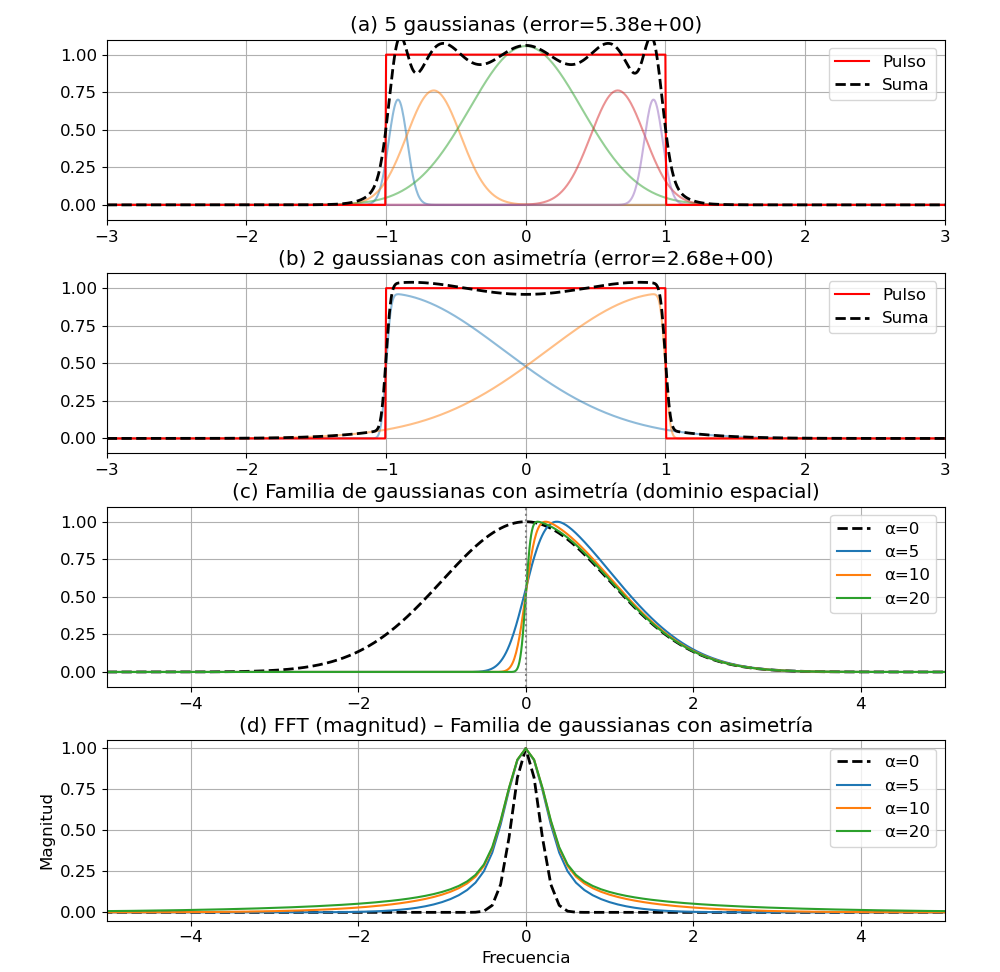
\includegraphics[width=1\textwidth]{Graphics/square_fft.png}
    \caption{Comparación entre gaussianas normales y gaussianas con asimetría en la aproximación de una señal cuadrada y sus respectivas transformadas de Fourier.   
    (a): Aproximación de un pulso cuadrado mediante la superposición de \(N = 5\) gaussianas simétricas optimizadas (error = 5.38). 
    (b): Aproximación del mismo pulso usando únicamente \(N = 2\) gaussianas con asimetría (error = 2.68), logrando una mejor representación de los bordes con menos componentes. 
    (c): Familia de gaussianas con diferentes niveles de asimetría en el dominio espacial para varios valores del parámetro \(\alpha\). A medida que \(\alpha\) aumenta, las funciones se inclinan hacia un lado, permitiendo mayor flexibilidad en la aproximación de funciones no simétricas. 
    (d): Magnitud de la transformada de Fourier (FFT) correspondiente a las funciones mostradas en (c), donde se observa que las gaussianas con asimetría presentan un mayor ancho de banda, lo que las hace más aptas para capturar componentes de alta frecuencia presentes en señales con transiciones abruptas.}
    \label{fig:square}
\end{figure}


\section{Estructura de la Tesis}
La tesis se organiza en los siguientes capítulos:
\begin{itemize}
    \item \textbf{Capítulo 2: Marco Teórico.} Se presentan conceptos fundamentales sobre espacios gaussianos, proyección y rasterización diferenciable, 
    y propiedades de distribuciones asimétricas.
    \item \textbf{Capítulo 3: Estado del Arte.} Se realiza una revisión crítica de \textit{Gaussian Splatting} y otros métodos relacionados, incluyendo técnicas 
    previas que abordan la modificación de las primitivas geométricas.
    \item \textbf{Capítulo 4: Metodología Propuesta.} Se detallan los aspectos teóricos y prácticos de la solución propuesta, incluyendo la simulación 
    de la asimetría y análisis de complejidad computacional.
    \item \textbf{Capítulo 5: Detalles de Implementación.} Se describen los componentes principales del código, incluyendo los kernels forward y backward 
    utilizados en el algoritmo de rasterización diferenciable propuesto.
    \item \textbf{Capítulo 6: Experimentos.} Se presentan hipótesis, diseño experimental, métricas de evaluación y resultados obtenidos tanto cuantitativos 
    como cualitativos.
    \item \textbf{Conclusiones y Recomendaciones.} Se resumen los aportes principales, limitaciones, aplicaciones potenciales y líneas futuras de 
    investigación sugeridas.
\end{itemize}
